\documentclass[11pt,letterpaper]{article}

%\usepackage{times}
%\usepackage{epsfig}
\usepackage{graphicx}
%\usepackage{amsmath}
%\usepackage{amssymb}
\usepackage{hyperref}
\usepackage{tabularx}
\usepackage[left=1in, right=1in, top=1in, bottom=1in]{geometry}
\usepackage{titling}
\usepackage{setspace}
\usepackage{sectsty}
\usepackage{tabto}
\graphicspath{{./Assignment_03_NOTEBOOK_Geidel_files/}} % adds the assets directory to the path, throw your images there
\usepackage{fancyhdr}
\pagestyle{fancy}
\fancyhf{}
\fancyheadoffset{0cm}
\renewcommand{\headrulewidth}{0pt} 
\renewcommand{\footrulewidth}{0pt}
\fancyhead[R]{\thepage}
\fancypagestyle{plain}{%
  \fancyhf{}%
  \fancyhead[R]{\thepage}%
}

\usepackage{cite}
\usepackage[sectionbib]{natbib}
\renewcommand{\refname}{}

\begin{document}
\fontfamily{ptm}\selectfont
\sectionfont{\fontsize{12}{12}\fontfamily{ptm}\selectfont}
\doublespacing
%%%%%%%%%%%%%%%%%%%%%%%%%%%%%% TITLE %%%%%%%%%%%%%%%%%%%%%%%%%%%%%%%%%%%%%%
\setlength{\droptitle}{1in} 

\title{\large{ASSIGNMENT 3: \\ INSURANCE POLICY \& CLAIMS AGENT \\\vspace{1.2in}}}

\author{
Kevin Geidel \\
MSDS 442: AI Agent Design \& Development \\
Northwestern University \\
May 18, 2025 \\
}

\date{}
\maketitle
\thispagestyle{empty}	
\clearpage
\setcounter{page}{1}

%%%%%%%%%%%%%%%%%%%%%%%%%%%%%% PAGE 1 %%%%%%%%%%%%%%%%%%%%%%%%%%%%%%%%%%%%

\section*{Requirement 1: Graph the agent with LangChain/LangGraph}
\tab The construction of the agent and accompanying graph begins with the creation of the functions that serve as edges in our graph (see cell 3 in the appendix). 
The actual assembly of the graph itself occurs in cell 9. However, some of the components, such as the conditional edge, \texttt{verify\_policy}, and \textbf{ClaimState} class,
are built above. Following the logic in cell 9 we first instantiate an empty graph:

\begin{verbatim}
workflow = StateGraph(AgentState)
\end{verbatim}

The \texttt{workflow} object has \texttt{add\_node} and \texttt{add\_edge} methods that allow us to assemble the 
components created in cells 3-8. The output is displayed graphically in cell 10 (reproduced in figure \ref{fig:graph} below.)

\begin{figure}[h!]
    \centering
    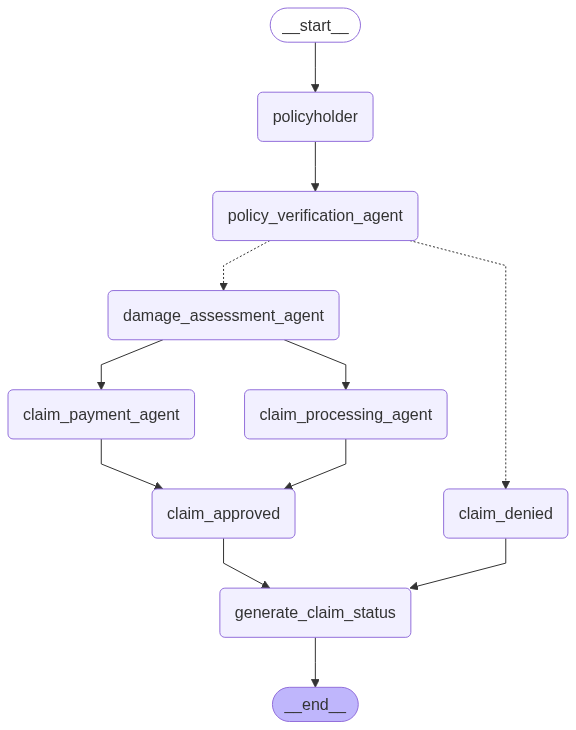
\includegraphics[height=400pt]{Assignment_03_NOTEBOOK_Geidel_9_0.png}
    \caption{Graphical depiction of the Allstate insurance policy and claims agent.}
    \label{fig:graph}
\end{figure}

\clearpage

\section*{Requirement 2: Establish desired process workflow}
\tab To meet the assignment objectives our agent must follow the provided workflow (shown in figure \ref{fig:bpmn}.)
Careful comparison of figures \ref{fig:graph} and \ref{fig:bpmn} show that each agent is represented as a node in the graph, 
decision formulated as a conditional and each function constructed as an edge. The workflow (depicted in \textit{Business Process Model Notion} or \textit{BPMN}) was provided to us for this assignment. However, construction of such a graphic is key for capturing all desired functionality and provides a map for the developer as they assemble the AI agents. In the figure we see each agent as its own swim lane and place the various decisions and actions into their respective spheres. Each bullet point in the requirements appears somewhere in this visual and acts as a checklist for the developer.

\begin{figure}[h!]
    \centering
    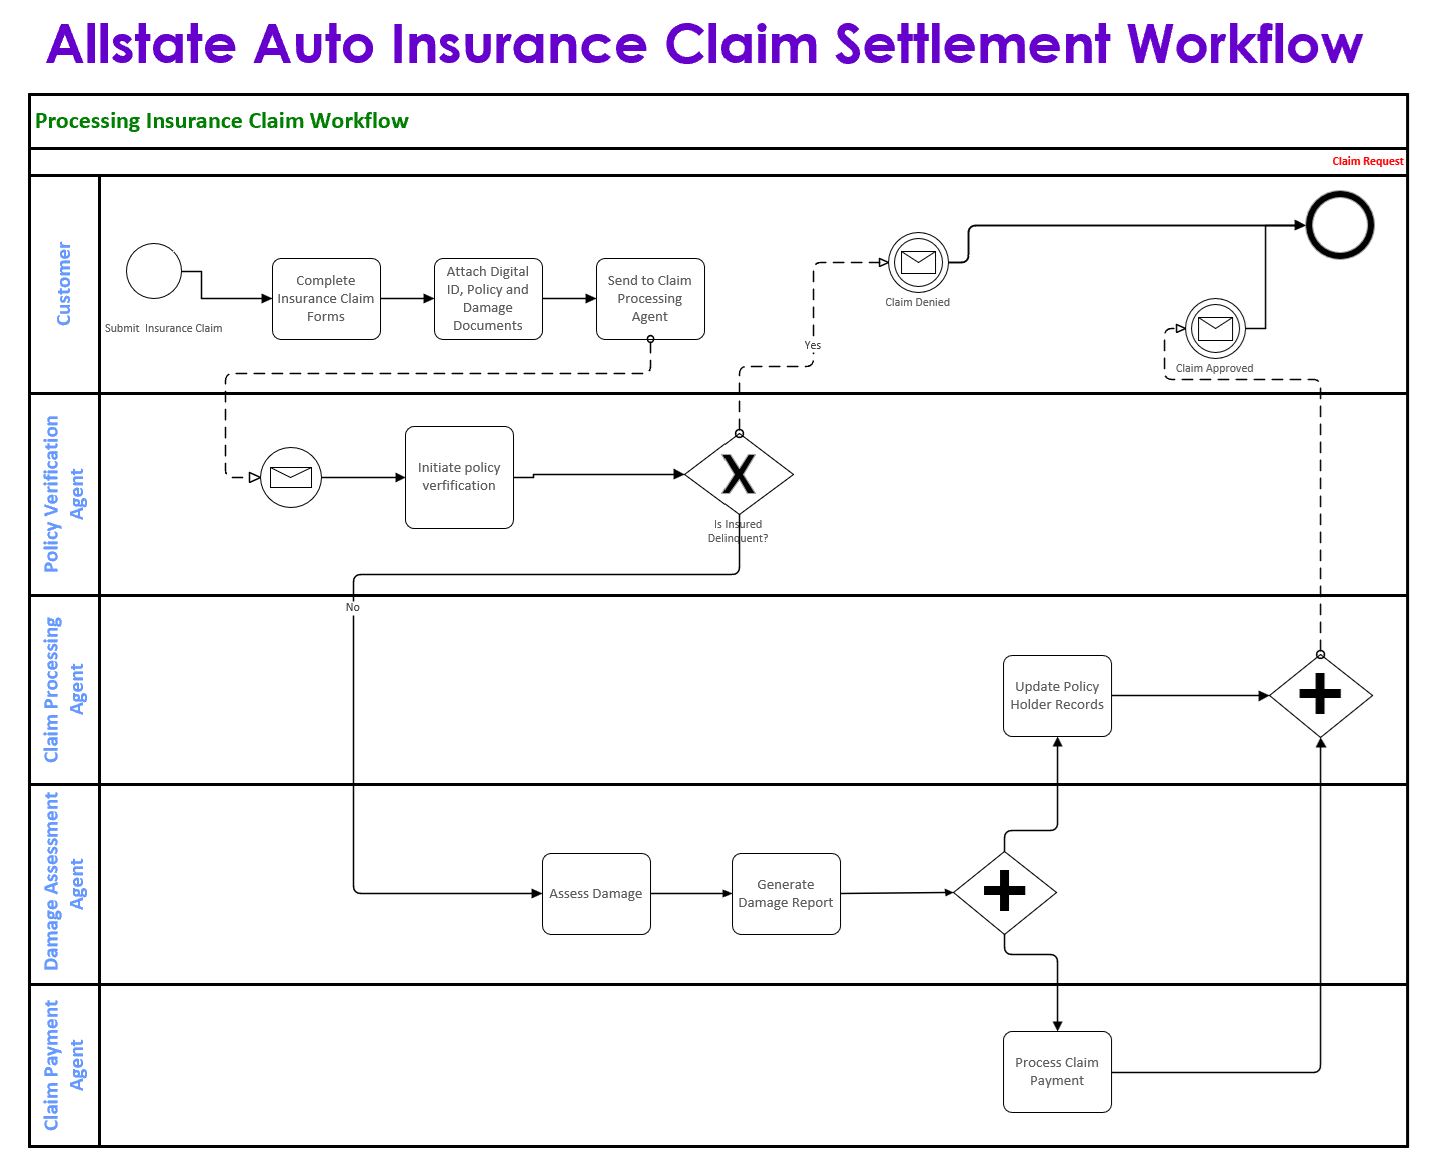
\includegraphics{BPMN.png}
    \caption{Desired agent workflow in \textit{Business Process Model Notation} (BPMN).}
    \label{fig:bpmn}
\end{figure}

\section*{Requirement 3: Prepare for expected user input}
\tab The user will provide their policy number and a photograph of the damage to their car. In preparation for this multi-modal inputs we build utilities for handling and displaying files in pdf format (cell 2.) A user's policy is loaded in cell 4 for use by the \texttt{policy\_verification\_agent}. 
In cell 5 we demonstrate the loading and display of an example vehicle damage photo. The trials in requirement 7 demonstrate the agent's ability to receive these inputs and perform the desired analysis.

\section*{Requirement 4: The policy verification agent}
\tab The details on the policy pdf must be extracted and analyzed to ensure the customer had a valid policy that is current. 
The \texttt{policy\_verification\_agent} will examine these files and locate information required to make this decision. 
The core logic in the verification agent begins in cell 3 (reproduced below in cell \ref{fig:cell3}). 

\begin{figure}[h!]
    \centering
    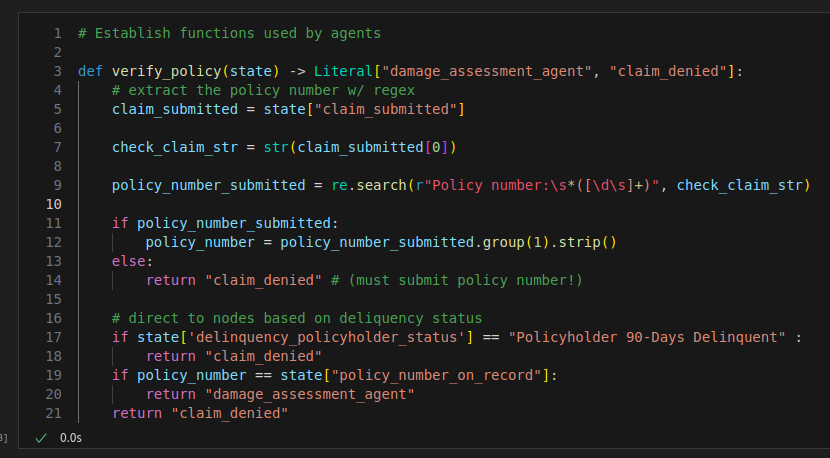
\includegraphics[width=1.0\linewidth]{cell_3.png}
    \caption{The \texttt{policy\_verification\_agent}.}
    \label{fig:cell3}
\end{figure}

\clearpage

\section*{Requirement 5: Process damage photo}
\tab Processing and analyzing the user's photo of vehicle damage is the job of the \texttt{damage\_assessment\_agent}. 
The logic used within the node occurs in cell 8. Many nodes and edges are instantiated in this cell but in figure \ref{fig:damage}
we focus on the query that will have the LLM rank the level of damage shown in the photo.

\begin{figure}[h!]
    \centering
    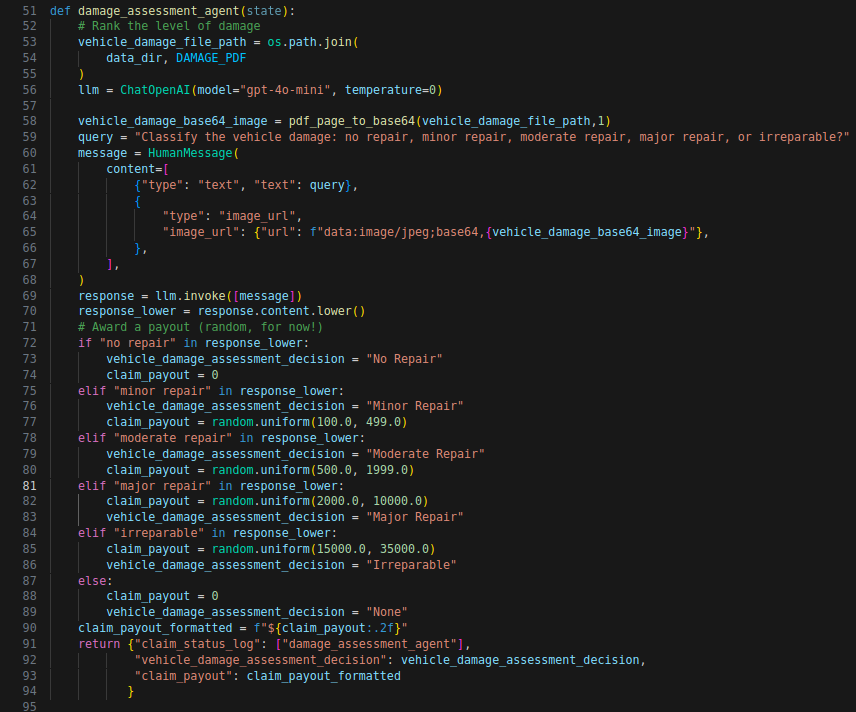
\includegraphics[width=0.75\linewidth]{damage_assessment_agent.png}
    \caption{The \texttt{damage\_assessment\_agent}.}
    \label{fig:damage}
\end{figure}

\section*{Requirement 6: The claim processing agent}
\tab The \texttt{claim\_processing\_agent} ensures that the decision letter is stamped with the proper dates.
Assignment requirements described a seven day delay between approval and disbursement (see cell 8.)

\section*{Requirement 7: Trial runs}
\tab The agents were tested under several conditions. Each scenario is described with a comment at the top of their respective cell.
The output is the Markdown formatted decision letter that is returned to the user. The queries and their outputs are shown in cells 12 through 16.



\end{document}